\documentclass[12pt, a4paper]{article}

\usepackage[utf8]{inputenc}
\usepackage{geometry}
\usepackage{graphicx}
\usepackage{tikz}
\usepackage{tabularx}
\usepackage{multicol}
\usepackage{multirow}
\usepackage{array,booktabs,ragged2e}
\usepackage{amsmath}
\usepackage{xkeyval}
\usepackage{float}
\usepackage{physics}
\usepackage{tfrupee}
\usepackage{mathtools} %underbrace symbol
\usepackage{adjustbox} 
\usepackage{xcolor}
\usepackage{colortbl}
\usepackage{tkz-euclide}
\usepackage{pgf-pie}
\usepackage[misc]{ifsym} %Used in tally mark
\usetikzlibrary{patterns,calc}

\newcommand{\scalefactor}{1}


\geometry{top=2.5cm, bottom=1.25cm, left=1.5cm, right=1.5cm}
\makeatletter
%-----------------------------------------------------------
% text bottom 4 option in 1 row
%-----------------------------------------------------------

\define@key{mcqtextbottomFourOne}{questionnumber}{\def\mcqtextbottomFourOnequestionnumber{#1}} 
\define@key{mcqtextbottomFourOne}{questionTag}{\def\mcqtextbottomFourOnequestionTag{#1}}
\define@key{mcqtextbottomFourOne}{questiontext}{\def\mcqtextbottomFourOnequestiontext{#1}}
\define@key{mcqtextbottomFourOne}{optionA}{\def\mcqtextbottomFourOneoptionA{#1}}
\define@key{mcqtextbottomFourOne}{optionB}{\def\mcqtextbottomFourOneoptionB{#1}}
\define@key{mcqtextbottomFourOne}{optionC}{\def\mcqtextbottomFourOneoptionC{#1}}
\define@key{mcqtextbottomFourOne}{optionD}{\def\mcqtextbottomFourOneoptionD{#1}}
\define@key{mcqtextbottomFourOne}{correctoption}{\def\mcqtextbottomFourOnecorrectoption{#1}}


\newcommand{\mcqtextbottomFourOne}[1]{%
\setkeys{mcqtextbottomFourOne}{#1}%
\vspace{2.5mm}
\begin{raggedright}
\textbf{Question Tag:} \mcqtextbottomFourOnequestionTag \hfill \textbf{Correct Option:} \mcqtextbottomFourOnecorrectoption\\
\end{raggedright}
\vspace{\baselineskip}
\begin{raggedright}
\textbf{Question \mcqtextbottomFourOnequestionnumber:} \mcqtextbottomFourOnequestiontext\\
\medskip
(a) \medskip \mcqtextbottomFourOneoptionA\\
(b) \medskip \mcqtextbottomFourOneoptionB\\      
(c) \medskip \mcqtextbottomFourOneoptionC\\
(d) \medskip \mcqtextbottomFourOneoptionD\\
\end{raggedright}
}

%-----------------------------------------------------------

%-----------------------------------------------------------

% DEFINE KEY FOR mcqtextbottomOneFour %

\define@key{mcqtextbottomOneFour}{questionnumber}{\def\mcqtextbottomOneFourquestionnumber{#1}} 
\define@key{mcqtextbottomOneFour}{questiontext}{\def\mcqtextbottomOneFourquestiontext{#1}}
\define@key{mcqtextbottomOneFour}{optionA}{\def\mcqtextbottomOneFouroptionA{#1}}
\define@key{mcqtextbottomOneFour}{optionB}{\def\mcqtextbottomOneFouroptionB{#1}}
\define@key{mcqtextbottomOneFour}{optionC}{\def\mcqtextbottomOneFouroptionC{#1}}
\define@key{mcqtextbottomOneFour}{optionD}{\def\mcqtextbottomOneFouroptionD{#1}}
\define@key{mcqtextbottomOneFour}{questionTag}{\def\mcqtextbottomOneFourquestionTag{#1}} 
\define@key{mcqtextbottomOneFour}{correctoption}{\def\mcqtextbottomOneFourcorrectoption{#1}}

% COMMAND FOR mcqtextbottomOneFour %

\newcommand{\mcqtextbottomOneFour}[1]{%
\setkeys{mcqtextbottomOneFour}{#1}%
\vspace{2.5mm}
\begin{raggedright}
\textbf{Question Tag:} \mcqtextbottomOneFourquestionTag \hfill \textbf{Correct Option:} \mcqtextbottomOneFourcorrectoption\\
\end{raggedright}
\vspace{\baselineskip}
\begin{raggedright}
\textbf{Question \mcqtextbottomOneFourquestionnumber:} \mcqtextbottomOneFourquestiontext
\begin{multicols}{4}
(a) \medskip \mcqtextbottomOneFouroptionA\\
(b) \medskip \mcqtextbottomOneFouroptionB\\      
(c) \medskip \mcqtextbottomOneFouroptionC\\
(d) \medskip \mcqtextbottomOneFouroptionD\\
\end{multicols}
\end{raggedright}
}

%-----------------------------------------------------------

%-----------------------------------------------------------

% Define key FOR mcqtextbottomOneTwo 

\define@key{mcqtextbottomOneTwo}{questionnumber}{\def\mcqtextbottomOneTwoquestion{#1}}
\define@key{mcqtextbottomOneTwo}{questiontext}{\def\mcqtextbottomOneTwoquestiontext{#1}}
\define@key{mcqtextbottomOneTwo}{optionA}{\def\mcqtextbottomOneTwooptionA{#1}}
\define@key{mcqtextbottomOneTwo}{optionB}{\def\mcqtextbottomOneTwooptionB{#1}}
\define@key{mcqtextbottomOneTwo}{questionTag}{\def\mcqtextbottomOneTwoquestionTag{#1}}
\define@key{mcqtextbottomOneTwo}{correctoption}{\def\mcqtextbottomOneTwocorrectoption{#1}}

% COMMAND FOR mcqtextbottomOneTwo %

\newcommand{\mcqtextbottomOneTwo}[1]{%
\setkeys{mcqtextbottomOneTwo}{#1}%
\vspace{2.5mm}
\begin{raggedright}
\textbf{Question Tag:} \mcqtextbottomOneTwoquestionTag \hfill \textbf{Correct Option:} \mcqtextbottomOneTwocorrectoption\\
\end{raggedright}
\vspace{\baselineskip}
\begin{raggedright}
\textbf{Question \mcqtextbottomOneTwoquestion:} \mcqtextbottomOneTwoquestiontext\\
\begin{multicols}{2}
(a) \medskip \mcqtextbottomOneTwooptionA\\
(b) \medskip \mcqtextbottomOneTwooptionB\\
\end{multicols}
\end{raggedright}
}

%-----------------------------------------------------------

%-----------------------------------------------------------

% Define key FOR mcqtextbottomTwoTwo

\define@key{mcqtextbottomTwoTwo}{questionnumber}{\def\mcqtextbottomTwoTwoquestion{#1}}
\define@key{mcqtextbottomTwoTwo}{questiontext}{\def\mcqtextbottomTwoTwoquestiontext{#1}}
\define@key{mcqtextbottomTwoTwo}{optionA}{\def\mcqtextbottomTwoTwooptionA{#1}}
\define@key{mcqtextbottomTwoTwo}{optionB}{\def\mcqtextbottomTwoTwooptionB{#1}}
\define@key{mcqtextbottomTwoTwo}{optionC}{\def\mcqtextbottomTwoTwooptionC{#1}}
\define@key{mcqtextbottomTwoTwo}{optionD}{\def\mcqtextbottomTwoTwooptionD{#1}}
\define@key{mcqtextbottomTwoTwo}{questionTag}{\def\mcqtextbottomTwoTwoquestionTag{#1}}
\define@key{mcqtextbottomTwoTwo}{correctoption}{\def\mcqtextbottomTwoTwocorrectoption{#1}}

% COMMAND FOR mcqtextbottomTwoTwo %

\newcommand{\mcqtextbottomTwoTwo}[1]{%
\setkeys{mcqtextbottomTwoTwo}{#1}%
\vspace{1.5mm}
\begin{raggedright}
\textbf{Question Tag:} \mcqtextbottomTwoTwoquestionTag \hfill \textbf{Correct Option:} \mcqtextbottomTwoTwocorrectoption\\
\end{raggedright}
\vspace{\baselineskip}
\begin{raggedright}
\textbf{Question \mcqtextbottomTwoTwoquestion:} \mcqtextbottomTwoTwoquestiontext\\
\begin{multicols}{2}
(a) \medskip \mcqtextbottomTwoTwooptionA\\
(c) \medskip \mcqtextbottomTwoTwooptionC\\
\columnbreak
(b) \medskip \mcqtextbottomTwoTwooptionB\\
(d) \medskip \mcqtextbottomTwoTwooptionD\\
\end{multicols}
\end{raggedright}
\vspace{5mm}
}

%-----------------------------------------------------------

%-----------------------------------------------------------

% Define key FOR mcqtextsideFourOne


\define@key{mcqtextsideFourOne}{questionnumber}{\def\mcqtextsideFourOnequestionnumber{#1}} 
\define@key{mcqtextsideFourOne}{questionTag}{\def\mcqtextsideFourOnequestionTag{#1}} 
\define@key{mcqtextsideFourOne}{questiontext}{\def\mcqtextsideFourOnequestiontext{#1}}
\define@key{mcqtextsideFourOne}{optionA}{\def\mcqtextsideFourOneoptionA{#1}}
\define@key{mcqtextsideFourOne}{optionB}{\def\mcqtextsideFourOneoptionB{#1}}
\define@key{mcqtextsideFourOne}{optionC}{\def\mcqtextsideFourOneoptionC{#1}}
\define@key{mcqtextsideFourOne}{optionD}{\def\mcqtextsideFourOneoptionD{#1}}
\define@key{mcqtextsideFourOne}{correctoption}{\def\mcqtextsideFourOnecorrectoption{#1}}
\define@key{mcqtextsideFourOne}{leftmini}{\def\mcqtextsideFourOneleftmini{#1}}
\define@key{mcqtextsideFourOne}{rightmini}{\def\mcqtextsideFourOnerightmini{#1}}

% COMMAND FOR mcqtextsideFourOne

\newcommand{\mcqtextsideFourOne}[1]{%
\setkeys{mcqtextsideFourOne}{#1}%
\vspace{2.5mm}
\begin{raggedright}
\textbf{Question Tag:} \mcqtextsideFourOnequestionTag \hfill \textbf{Correct Option:} \mcqtextsideFourOnecorrectoption\\
\end{raggedright}
\vspace{\baselineskip}
\begin{raggedright}
\begin{minipage}[t]{\mcqtextsideFourOneleftmini\linewidth}
\textbf{Question \mcqtextsideFourOnequestionnumber:} \mcqtextsideFourOnequestiontext\\
\end{minipage}\hfill
\begin{minipage}[t]{\mcqtextsideFourOnerightmini\linewidth}
(a) \medskip \mcqtextsideFourOneoptionA\\
(b) \medskip \mcqtextsideFourOneoptionB\\
(c) \medskip \mcqtextsideFourOneoptionC\\
(d) \medskip \mcqtextsideFourOneoptionD\\
\end{minipage}
\end{raggedright}
}

%-----------------------------------------------------------

%-----------------------------------------------------------

% Define key FOR mcqimgbottomOneFour

\define@key{mcqimgbottomOneFour}{questionnumber}{\def\mcqimgbottomOneFourquestionnumber{#1}}
\define@key{mcqimgbottomOneFour}{questionTag}{\def\mcqimgbottomOneFourquestionTag{#1}}
\define@key{mcqimgbottomOneFour}{questiontext}{\def\mcqimgbottomOneFourquestiontext{#1}}
\define@key{mcqimgbottomOneFour}{optionA}{\def\mcqimgbottomOneFouroptionA{#1}}
\define@key{mcqimgbottomOneFour}{optionB}{\def\mcqimgbottomOneFouroptionB{#1}}
\define@key{mcqimgbottomOneFour}{optionC}{\def\mcqimgbottomOneFouroptionC{#1}}
\define@key{mcqimgbottomOneFour}{optionD}{\def\mcqimgbottomOneFouroptionD{#1}}
\define@key{mcqimgbottomOneFour}{correctoption}{\def\mcqimgbottomOneFourcorrectoption{#1}}

% COMMAND FOR mcqimgbottomOneFour %

\newcommand{\mcqimgbottomOneFour}[1]{%
\setkeys{mcqimgbottomOneFour}{#1}%
\vspace{2.5mm}
\begin{raggedright}
\textbf{Question Tag:} \mcqimgbottomOneFourquestionTag \hfill \textbf{Correct Option:} \mcqimgbottomOneFourcorrectoption\\
\end{raggedright}
\vspace{\baselineskip}
\begin{raggedright}
\textbf{Question \mcqimgbottomOneFourquestionnumber:} \mcqimgbottomOneFourquestiontext \\
\begin{multicols}{4}
(a) \includegraphics[width=3cm, height=2.5cm]{\mcqimgbottomOneFouroptionA}  \\
(b) \includegraphics[width=3cm, height=2.5cm]{\mcqimgbottomOneFouroptionB}   \\
(c) \includegraphics[width=3cm, height=2.5cm]{\mcqimgbottomOneFouroptionC}  \\
(d) \includegraphics[width=3cm, height=2.5cm]{\mcqimgbottomOneFouroptionD} 
\end{multicols}
\end{raggedright}
}

%-----------------------------------------------------------

%-----------------------------------------------------------

% Define key FOR mcqimgdbottomOneFour

\define@key{mcqimgdbottomOneFour}{questionnumber}{\def\mcqimgdbottomOneFourquestionnumber{#1}}
\define@key{mcqimgdbottomOneFour}{questionTag}{\def\mcqimgdbottomOneFourquestionTag{#1}}
\define@key{mcqimgdbottomOneFour}{questiontext}{\def\mcqimgdbottomOneFourquestiontext{#1}}
\define@key{mcqimgdbottomOneFour}{optionA}{\def\mcqimgdbottomOneFouroptionA{#1}}
\define@key{mcqimgdbottomOneFour}{optionAtext}{\def\mcqimgdbottomOneFouroptionAtext{#1}}
\define@key{mcqimgdbottomOneFour}{optionB}{\def\mcqimgdbottomOneFouroptionB{#1}}
\define@key{mcqimgdbottomOneFour}{optionBtext}{\def\mcqimgdbottomOneFouroptionBtext{#1}}
\define@key{mcqimgdbottomOneFour}{optionC}{\def\mcqimgdbottomOneFouroptionC{#1}}
\define@key{mcqimgdbottomOneFour}{optionCtext}{\def\mcqimgdbottomOneFouroptionCtext{#1}}
\define@key{mcqimgdbottomOneFour}{optionD}{\def\mcqimgdbottomOneFouroptionD{#1}}
\define@key{mcqimgdbottomOneFour}{optionDtext}{\def\mcqimgdbottomOneFouroptionDtext{#1}}
\define@key{mcqimgdbottomOneFour}{correctoption}{\def\mcqimgdbottomOneFourcorrectoption{#1}}

% COMMAND FOR mcqimgdbottomOneFour %

\newcommand{\mcqimgdbottomOneFour}[1]{%
\setkeys{mcqimgdbottomOneFour}{#1}%
\vspace{2.5mm}
\begin{raggedright}
\textbf{Question Tag:} \mcqimgdbottomOneFourquestionTag \hfill \textbf{Correct Option:} \mcqimgdbottomOneFourcorrectoption\\
\end{raggedright}
\vspace{\baselineskip}
\begin{raggedright}
\textbf{Question \mcqimgdbottomOneFourquestionnumber:} \mcqimgdbottomOneFourquestiontext \\
\begin{multicols}{4}
\includegraphics[width=3cm, height=3cm]{\mcqimgdbottomOneFouroptionA} \\*
(a) \mcqimgdbottomOneFouroptionAtext \\

\includegraphics[width=3cm, height=3cm]{\mcqimgdbottomOneFouroptionB}  \\*     
(b) \mcqimgdbottomOneFouroptionBtext \\

\includegraphics[width=3cm, height=3cm]{\mcqimgdbottomOneFouroptionC} \\*
(c) \mcqimgdbottomOneFouroptionCtext \\

\includegraphics[width=3cm, height=3cm]{\mcqimgdbottomOneFouroptionD} \\*
(d) \mcqimgdbottomOneFouroptionDtext
\end{multicols}
\end{raggedright}
}

%-----------------------------------------------------------

%-----------------------------------------------------------

% Define key FOR mcqimgleftFourOne

\define@key{mcqimgleftFourOne}{questionnumber}{\def\mcqimgleftFourOnequestionnumber{#1}} 
\define@key{mcqimgleftFourOne}{questiontext}{\def\mcqimgleftFourOnequestiontext{#1}}
\define@key{mcqimgleftFourOne}{imgtabletikz}{\def\mcqimgtabletikz{#1}}
\define@key{mcqimgleftFourOne}{optionA}{\def\mcqimgleftFourOneoptionA{#1}}
\define@key{mcqimgleftFourOne}{optionB}{\def\mcqimgleftFourOneoptionB{#1}}
\define@key{mcqimgleftFourOne}{optionC}{\def\mcqimgleftFourOneoptionC{#1}}
\define@key{mcqimgleftFourOne}{optionD}{\def\mcqimgleftFourOneoptionD{#1}}
\define@key{mcqimgleftFourOne}{questionTag}{\def\mcqimgleftFourOnequestionTag{#1}} 
\define@key{mcqimgleftFourOne}{correctoption}{\def\mcqimgleftFourOnecorrectoption{#1}}
\define@key{mcqimgleftFourOne}{leftmini}{\def\mcqimgleftFourOneleftmini{#1}}
\define@key{mcqimgleftFourOne}{rightmini}{\def\mcqimgleftFourOnerightmini{#1}}

% COMMAND FOR mcqimgleftFourOne 

\newcommand{\mcqimgleftFourOne}[1]{%
\setkeys{mcqimgleftFourOne}{#1}%
\vspace{1.5mm}
\begin{raggedright}
\textbf{Question Tag:} \mcqimgleftFourOnequestionTag \hfill \textbf{Correct Option:} \mcqimgleftFourOnecorrectoption\\
\end{raggedright}
\vspace{\baselineskip}
\begin{raggedright}
\textbf{Question \mcqimgleftFourOnequestionnumber:} \mcqimgleftFourOnequestiontext\\
\medskip
\end{raggedright}
\begin{minipage}[]{\mcqimgleftFourOneleftmini\linewidth}
\Centering
\mcqimgtabletikz 
\end{minipage}\hfill
\begin{minipage}[]{\mcqimgleftFourOnerightmini\linewidth}
(a) \medskip \mcqimgleftFourOneoptionA\\
(b) \medskip \mcqimgleftFourOneoptionB\\
(c) \medskip \mcqimgleftFourOneoptionC\\
(d) \medskip \mcqimgleftFourOneoptionD\\      
\end{minipage}
\vspace{5mm}
}

%-----------------------------------------------------------

%-----------------------------------------------------------

% DEFINE KEY FOR mcqfourimg %

\define@key{mcqimgsideFourOne}{questionnumber} {\def\mcqimgsideFourOnequestionnumber{#1} }
\define@key{mcqimgsideFourOne}{questiontext}{\def\mcqimgsideFourOnequestiontext{#1}}
\define@key{mcqimgsideFourOne}{imgwidth}{\def\mcqimgsideFourOnewidth{#1}}
\define@key{mcqimgsideFourOne}{imgheight}{\def\mcqimgsideFourOneheight{#1}}
\define@key{mcqimgsideFourOne}{img}{\def\mcqimgsideFourOne{#1}}
\define@key{mcqimgsideFourOne}{optionA}{\def\mcqimgsideFourOneoptionA{#1}}
\define@key{mcqimgsideFourOne}{optionB}{\def\mcqimgsideFourOneoptionB{#1}}
\define@key{mcqimgsideFourOne}{optionC}{\def\mcqimgsideFourOneoptionC{#1}}
\define@key{mcqimgsideFourOne}{optionD}{\def\mcqimgsideFourOneoptionD{#1}}
\define@key{mcqimgsideFourOne}{questionTag}{\def\mcqimgsideFourOnequestionTag{#1}} 
\define@key{mcqimgsideFourOne}{correctoption}{\def\mcqimgsideFourOnecorrectoption{#1}}
\define@key{mcqimgsideFourOne}{leftmini}{\def\mcqimgsideFourOneleftmini{#1}}
\define@key{mcqimgsideFourOne}{rightmini}{\def\mcqimgsideFourOnerightmini{#1}}

\newcommand{\mcqimgsideFourOne}[1]{
\setkeys{mcqimgsideFourOne}{#1}
\vspace{2.5mm}
\begin{raggedright}
\textbf{Question Tag:} \mcqimgsideFourOnequestionTag \hfill \textbf{Correct Option:} \mcqimgsideFourOnecorrectoption \\
\end{raggedright}
\vspace{\baselineskip}
\begin{raggedright}
\begin{minipage}[]{\mcqimgsideFourOneleftmini\textwidth}
\textbf{Question \mcqimgsideFourOnequestionnumber:} \mcqimgsideFourOnequestiontext
\vspace{2mm} \\
(a) \medskip \mcqimgsideFourOneoptionA \\
(b) \medskip \mcqimgsideFourOneoptionB \\
(c) \medskip \mcqimgsideFourOneoptionC \\
(d) \medskip \mcqimgsideFourOneoptionD \\
\end{minipage}
\begin{minipage}[]{\mcqimgsideFourOnerightmini\textwidth}
\includegraphics[width=\mcqimgsideFourOnewidth, height=\mcqimgsideFourOneheight]{\mcqimgsideFourOne}
\end{minipage}
\end{raggedright}
\vspace{5mm}
}

%-----------------------------------------------------------
%               MCQ without Option
%-----------------------------------------------------------


\define@key{mcqdescriptive}{questionnumber}{\def\mcqdescriptivequestionnumber{#1}} 
\define@key{mcqdescriptive}{questionTag}{\def\mcqdescriptivequestionTag{#1}} 
\define@key{mcqdescriptive}{questiontext}{\def\mcqdescriptivequestiontext{#1}}
\define@key{mcqdescriptive}{correctoption}{\def\mcqdescriptivecorrectoption{#1}}

\newcommand{\mcqdescriptive}[1]{%
\setkeys{mcqdescriptive}{#1}%
\vspace{2.5mm}
\begin{raggedright}
\textbf{Question Tag:} \mcqdescriptivequestionTag \hfill \textbf{Correct Option:} \mcqdescriptivecorrectoption\\
\end{raggedright}
\vspace{\baselineskip}
\begin{raggedright}
\textbf{Question \mcqdescriptivequestionnumber:} \mcqdescriptivequestiontext
\end{raggedright}
\vspace{5mm}}

%-----------------------------------------------------------
%                        TABLE
%-----------------------------------------------------------
\newcolumntype{R}[1]{>{\Centering\arraybackslash}p{#1}}

\makeatother



\newcommand{\drawclock}[2]{
	\begin{tikzpicture}[scale=1]
		\draw[thick] (0,0) circle (1.5);
		\foreach \n in {1,...,12} {
			\node at ({1.2*sin(30*\n)}, {1.2*cos(30*\n)}) {\n};
		}
		\pgfmathsetmacro\hangle{90 - (#1 + #2/60)*30}
		\pgfmathsetmacro\mangle{90 - #2*6}
		\draw[thick] (0,0) -- ({0.7*cos(\hangle)}, {0.7*sin(\hangle)});
		\draw[thick] (0,0) -- ({1.2*cos(\mangle)}, {1.2*sin(\mangle)});
		\fill (0,0) circle (2pt);
	\end{tikzpicture}
}

\newcommand{\piechart}[1]{%
	\begin{tikzpicture}[scale=2.5]
		\def\start{90}
		\foreach \v/\l/\p/\c [count=\i] in {#1} {
			\pgfmathsetmacro\a{\v*3.6}
			\pgfmathsetmacro\mid{\start-\a/2}
			\coordinate (center) at (0,0);
			\coordinate (labelpt) at (\mid:1.3);
			\coordinate (percentpt) at (\mid:0.6);
			\fill[pattern=\p, pattern color=\c, draw=black] (center) -- (\start:1) arc (\start:\start-\a:1) -- cycle;
			\draw[black] (\mid:1) -- (\mid:1.2);
			\node at (labelpt) {\l};
			\node[fill=white, draw=black, rounded corners=1pt, inner sep=1pt] at (percentpt) {\v\%};
			\xdef\start{\start-\a}
		}
\end{tikzpicture}}

\graphicspath{ {C5M - Images/} {C5S - Images/} }

\begin{document}


%-----------------------------------------------------------
%                        Question [  ]
%-----------------------------------------------------------
% start-of-question
\mcqtextbottomOneFour{
questionnumber={10}, 
questionTag={C5M03 – DT – Q1},  
questiontext={Find the square that has one fourth shaded portion. },
optionA={
\adjustbox{scale=\scalefactor}{
\begin{tabular}{|c|c|c|c|}
		\hline
		\cellcolor{gray!50}& \\ \hline
		& \\ \hline
	\end{tabular} } },
optionB={
\adjustbox{scale=\scalefactor}{
\begin{tabular}{|c|c|c|c|}
		\hline
        \cellcolor{gray!50}	& \cellcolor{gray!50}\\ \hline
	  & \\ \hline
	\end{tabular} } },
optionC={
\adjustbox{scale=\scalefactor}{
\begin{tabular}{|c|c|c|c|}
		\hline
        \cellcolor{gray!50}	& \cellcolor{gray!50}\\ \hline
	  \cellcolor{gray!50}& \\ \hline
	\end{tabular} } },
optionD={
\adjustbox{scale=\scalefactor}{
\begin{tabular}{|c|c|c|c|}
		\hline
        \cellcolor{gray!50}	& \cellcolor{gray!50}\\ \hline
	  \cellcolor{gray!50}& \cellcolor{gray!50}\\ \hline
	\end{tabular} } },
correctoption={A},
}
% end-of-question

%-----------------------------------------------------------
%                        Question [  ]
%-----------------------------------------------------------
% start-of-question
\mcqtextbottomOneFour{
questionnumber={11}, 
questionTag={C5M03 – DT – Q3},  
questiontext={Find the fraction of shaded portions.\\
\medskip
\begin{center}
\adjustbox{scale=\scalefactor}{
\begin{tabular}{|p{1cm}|p{1cm}|p{1cm}|p{1cm}|p{1cm}|p{1cm}|p{1cm}|p{1cm}|p{1cm}|p{1cm}|}
	\hline
    \cellcolor{gray!50}	& \cellcolor{gray!50} & & & \\ \hline
	\cellcolor{gray!50}& \cellcolor{gray!50}& & & \\ \hline
\end{tabular}}
\end{center}},
optionA={$\frac{6}{10}$},
optionB={$\frac{2}{3}$},
optionC={$\frac{4}{6}$},
optionD={$\frac{4}{10}$},
correctoption={D},
}
% end-of-question

%-----------------------------------------------------------
%                        Question [  ]
%-----------------------------------------------------------
% start-of-question
\mcqimgleftFourOne{
questionnumber={15}, 
questionTag={C5M05 – DT – Q1}, 
questiontext={Identify the number of sides in the given figure.},
imgtabletikz = { 
\adjustbox{scale=\scalefactor}{
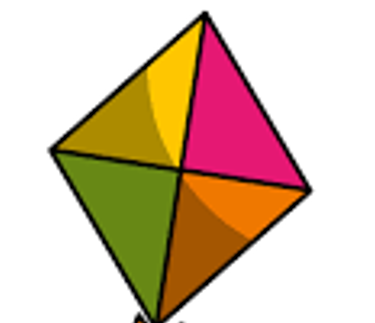
\includegraphics[height= 2.5cm, width= 3.5 cm]{C5M05 – DT – Q1.png}}
},
optionA={No sides},
optionB={Six sides},
optionC={Four sides},
optionD={Three sides},
correctoption={C},
leftmini={0.5},
rightmini={0.4},
}
% end-of-question
 
%-----------------------------------------------------------
%                        Question [  ]
%-----------------------------------------------------------
% start-of-question
\mcqimgleftFourOne{
questionnumber={17}, 
questionTag={C5M05 – DT – Q2},  
questiontext={Find the length of pencil. },
imgtabletikz = {
\adjustbox{scale=\scalefactor}{ 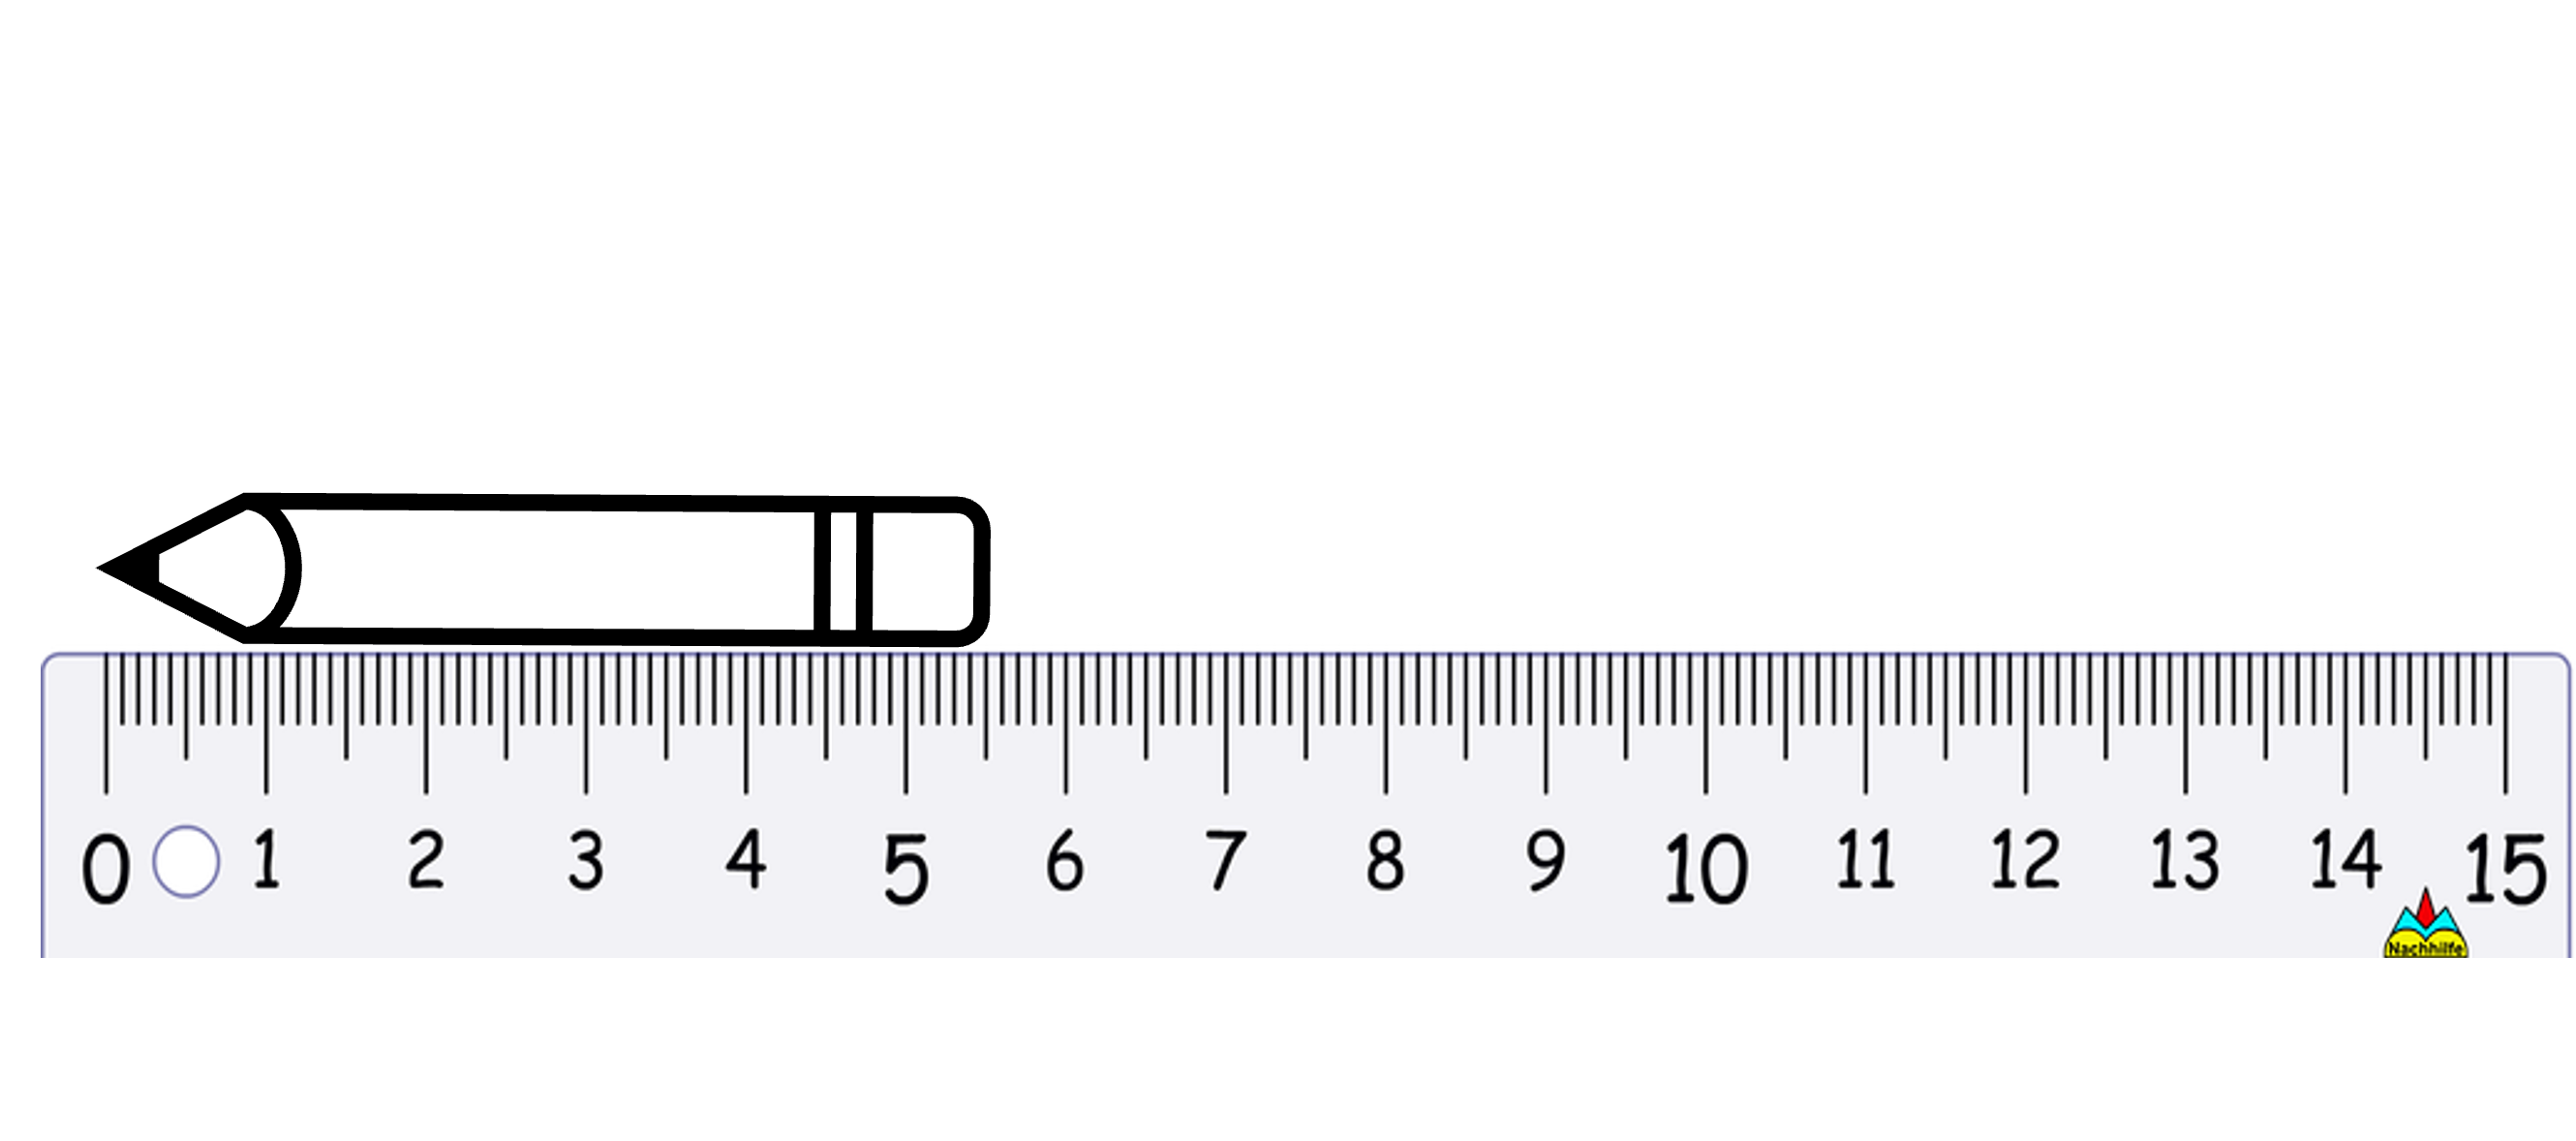
\includegraphics[height= 3cm, width= 10 cm]{C5M05 – DT – Q2.png}}},
optionA={6.5 cm},
optionB={5.5 cm},
optionC={5 cm},
optionD={6 cm},
correctoption={B},
leftmini={0.6},
rightmini={0.3},
}
% end-of-question

%-----------------------------------------------------------
%                        Question [  ]
%-----------------------------------------------------------
% start-of-question
\mcqimgleftFourOne{
questionnumber={18}, 
questionTag={C5M05 – DT – Q3},  
questiontext={In the given figure, the angle formed is \rule{80pt}{0.5pt} the right angle. },
imgtabletikz = {\adjustbox{scale=\scalefactor}{\drawclock{05}{00}}},
optionA={Equal to},
optionB={Greater than},
optionC={Lesser than},
optionD={Not equal to},
correctoption={B},
leftmini={0.6},
rightmini={0.3},
}
% end-of-question

%-----------------------------------------------------------
%                        Question [  ]
%-----------------------------------------------------------
% start-of-question
\mcqimgleftFourOne{
questionnumber={18}, 
questionTag={C5M08 – DT – Q1},  
questiontext={Find the area of the following shaded squares, if the side of one square is 1 cm. },
imgtabletikz = {
\adjustbox{scale=\scalefactor}{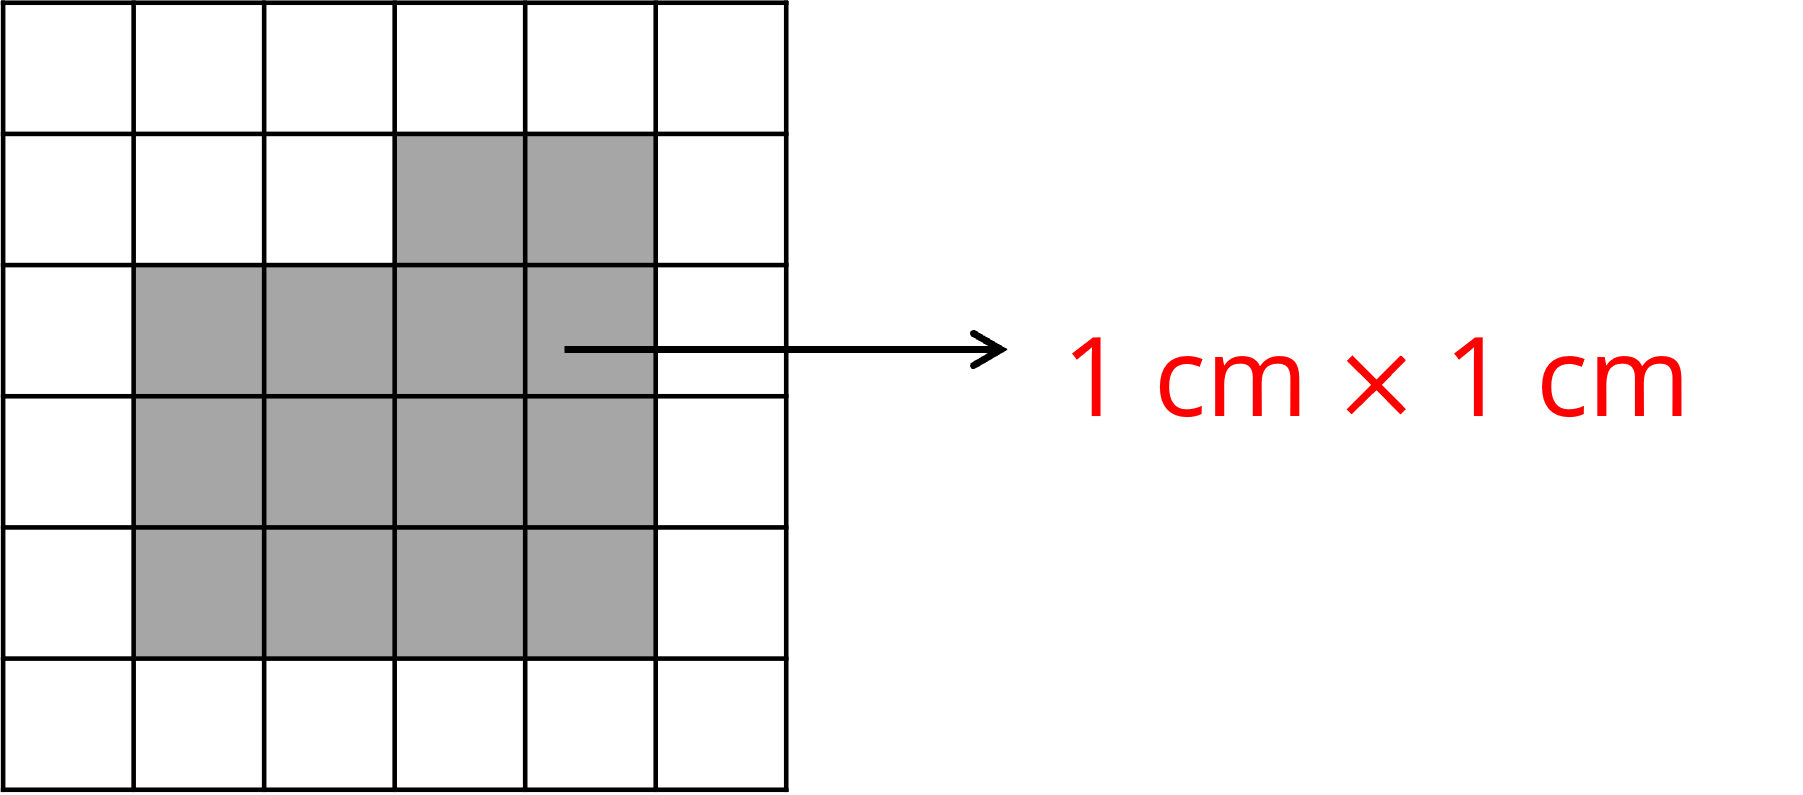
\includegraphics[height= 2.5cm, width= 6 cm]{C5M08 – DT – Q1.png}}},
optionA={28 sq. cm},
optionB={56 sq. cm},
optionC={14 sq. cm},
optionD={7 sq. cm},
correctoption={C},
leftmini={0.6},
rightmini={0.3},
}
% end-of-question

%-----------------------------------------------------------
%                        Question [  ]
%-----------------------------------------------------------
% start-of-question
\mcqimgleftFourOne{
questionnumber={20}, 
questionTag={C5M08 – DT – Q3},  
questiontext={Find the area of the rectangle. },
imgtabletikz = { 
\adjustbox{scale=\scalefactor}{
\begin{tikzpicture}
	\tkzDefPoint(0,0){A}
	\tkzDefPoint(4,0){B}
	\tkzDefPoint(4,2){C}
	\tkzDefPoint(0,2){D}
	\tkzDrawPolygon[fill=gray!50](A,B,C,D)
			
	\tkzLabelSegment[above](C,D){$20$ cm}
	\tkzLabelSegment[right](B,C){$8$ cm}
\end{tikzpicture} } },
optionA={12 sq. cm},
optionB={28 sq. cm},
optionC={56 sq. cm},
optionD={160 sq.cm},
correctoption={D},
leftmini={0.6},
rightmini={0.3},
}
% end-of-question

%-----------------------------------------------------------
%                        Question [  ]
%-----------------------------------------------------------
% start-of-question
\mcqtextbottomOneFour{
questionnumber={21}, 
questionTag={C5M07 – DT – Q2},  
questiontext={Pick the shape which is not divided into two mirror halves by the dotted line.\\
\adjustbox{scale=\scalefactor}{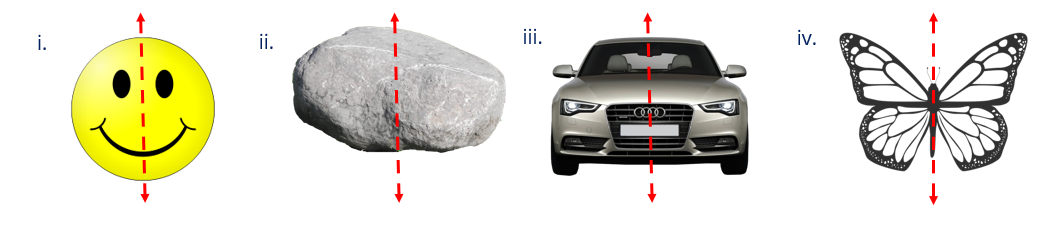
\includegraphics[height= 3.5cm, width= 16 cm]{C5M07 – DT – Q2.png}}
},
optionA={i},
optionB={ii},
optionC={iii},
optionD={iv},
correctoption={B},
}
% end-of-question

%-----------------------------------------------------------
%                        Question [  ]
%-----------------------------------------------------------
% start-of-question
\mcqimgleftFourOne{
questionnumber={23}, 
questionTag={C5M06 – DT – Q2},  
questiontext={ Identify the shape of the following image.},
imgtabletikz = { 
\adjustbox{scale=\scalefactor}{
\begin{tikzpicture}
	\tkzDefPoint(0,0){A}
	\tkzDefPoint(3,0){B}
	\tkzDefPoint(1.5,3){C}

	\tkzDrawSegment(A,C)
	\tkzDrawSegment(B,C)
	\draw[dashed] (A) arc[start angle=180,end angle=0,x radius=1.5,y radius=0.5];
	\draw (A) arc[start angle=180,end angle=360,x radius=1.5,y radius=0.5];
\end{tikzpicture} } },
optionA={Cube},
optionB={Cuboid},
optionC={Cone},
optionD={Cylinder},
correctoption={C},
leftmini={0.6},
rightmini={0.3},
}
% end-of-question

%-----------------------------------------------------------
%                        Question [  ]
%-----------------------------------------------------------
% start-of-question
\mcqtextbottomOneFour{
questionnumber={24}, 
questionTag={C5M09 – DT – Q1},  
questiontext={Find the number for the tally mark representation of \adjustbox{scale=\scalefactor}{ \scalebox{2}{\StrokeFive} \scalebox{2}{\StrokeOne} } },
optionA={8},
optionB={6},
optionC={7},
optionD={5},
correctoption={B},
}
% end-of-question

%-----------------------------------------------------------
%                        Question [  ]
%-----------------------------------------------------------
% start-of-question
\mcqimgleftFourOne{
questionnumber={25}, 
questionTag={C5M09 – DT – Q2},  
questiontext={Which genre is liked more? },
imgtabletikz = {\adjustbox{scale=\scalefactor}{ 
\piechart{
		5/Horror/north east lines/cyan,
		15/Action/dots/magenta,
		35/Comedy/crosshatch/green,
		25/Romance/bricks/teal,
		20/Thriller/grid/violet!50
	} } },
optionA={Comedy},
optionB={Horror},
optionC={Thriller},
optionD={Romance},
correctoption={A},
leftmini={0.6},
rightmini={0.3},
}
% end-of-question

%-----------------------------------------------------------
%                        Question [  ]
%-----------------------------------------------------------
% start-of-question
\mcqimgleftFourOne{
questionnumber={25}, 
questionTag={C5M09 – DT – Q2},  
questiontext={Which genre is liked more? },
imgtabletikz = {\adjustbox{scale=\scalefactor}{ 
\piechart{
		5/Horror/north east lines/cyan,
		15/Action/dots/magenta,
		35/Comedy/crosshatch/green,
		25/Romance/bricks/teal,
		20/Thriller/grid/violet!50
	} } },
optionA={Comedy},
optionB={Horror},
optionC={Thriller},
optionD={Romance},
correctoption={A},
leftmini={0.6},
rightmini={0.3},
}
% end-of-question

\end{document}